	\documentclass[aspectratio=43]{beamer}
\usepackage[english]{babel}
\usepackage{amsthm}
\usepackage{amsfonts}
\usepackage{amsmath}
\usepackage{amssymb}
\usepackage{mathtools}
\usepackage{bbm}
\usepackage{pgfplots}
\usepackage{tikz}
%\usepackage{physics}
\usepackage{calligra}
\usepackage{csquotes}
%\usepackage{tensor}
\usepackage[thicklines]{cancel}
\usepackage{tcolorbox}
%\usepackage{pstricks}
\usepackage[backend=biber, bibstyle=nature, sorting=nty, citestyle=numeric-comp]{biblatex} %Custom bibliography
    \addbibresource{bib.bib} %Load references
\usepackage{chronology}
\usepackage{msc}

\DeclareMathAlphabet{\mathcalligra}{T1}{calligra}{m}{n}
\DeclareFontShape{T1}{calligra}{m}{n}{<->s*[2.2]callig15}{}
\newcommand{\scriptr}{\mathcalligra{r}\,}
\newcommand{\boldscriptr}{\pmb{\mathcalligra{r}}\,}
\def\rc{\scriptr}
\def\brc{\boldscriptr}
\def\hrc{\hat\brc}
\newcommand{\ie}{\emph{i.e.}} %id est
\newcommand{\eg}{\emph{e.g.}} %exempli gratia
\newcommand{\rtd}[1]{\ensuremath{\left\lfloor #1 \right\rfloor}}
\newcommand{\dirac}[1]{\ensuremath{\delta \left( #1 \right)}}
\newcommand{\diract}[1]{\ensuremath{\delta^3 \left( #1 \right)}}
\newcommand{\e}{\ensuremath{\epsilon_0}}
\newcommand{\m}{\ensuremath{\mu_0}}
\newcommand{\V}{\ensuremath{\mathcal{V}}}
\newcommand{\prnt}[1]{\ensuremath{\left(#1\right)}} %parentheses
\newcommand{\colch}[1]{\ensuremath{\left[#1\right]}} %square brackets
\newcommand{\chave}[1]{\ensuremath{\left\{#1\right\}}}  %curly brackets
\newcommand\eqdef{\stackrel{\mathclap{\normalfont \tiny\mbox{\textrm{def}}}}{=}}
\useoutertheme{infolines}
\useinnertheme{rectangles}
\usefonttheme{professionalfonts}


\definecolor{blue2}{HTML}{045FB4}
\definecolor{green2}{HTML}{46C235}
\definecolor{red2}{HTML}{EE4848}
\definecolor{violet2}{HTML}{A647E5}
\definecolor{orange2}{HTML}{FF7425}
\definecolor{darkred}{HTML}{5C2020}
\definecolor{gray}{HTML}{303030}
\definecolor{yellow}{HTML}{f0be52}
\definecolor{lightdarkgold}{HTML}{EEBC1D}

\renewcommand{\CancelColor}{\color{darkred}}

\makeatletter
\newcommand{\mybox}[1]{%
  \setbox0=\hbox{#1}%
  \setlength{\@tempdima}{\dimexpr\wd0+13pt}%
  \begin{tcolorbox}[colback=gray,colframe=gray,boxrule=0.5pt,arc=4pt,
      left=6pt,right=6pt,top=6pt,bottom=6pt,boxsep=0pt,width=\@tempdima]
    \textcolor{yellow}{#1}
  \end{tcolorbox}
}
\makeatother


\pgfplotsset{my style/.append style={axis x line=middle, axis y line=
middle, xlabel={$x$}, ylabel={$y$}, axis equal }}


\usecolortheme[named=gray]{structure}
\usecolortheme{sidebartab}
\usecolortheme{orchid}
\usecolortheme{whale}
\setbeamercolor{titlelike}{parent=structure, bg=structure, fg=white}
\setbeamercolor{section in toc}{fg= white}
\setbeamercolor{subsection in toc}{fg= white}
%\setbeamercolor*{sidebar}{fg=red2,bg=gray!15!white}

\setbeamercolor{item projected}{bg=yellow, fg = gray}
\setbeamertemplate{enumerate items}[default]
\setbeamertemplate{navigation symbols}{}
\setbeamercolor{local structure}{fg=yellow}

\setbeamercolor{alerted text}{fg=white}
\setbeamercolor{block title}{bg = yellow}
\setbeamercolor{block title alerted}{bg=red2}
\setbeamercolor{block title example}{bg=green2}
\setbeamercolor{background canvas}{bg=gray}
\setbeamercolor{normal text}{bg=gray,fg=white}


\setbeamertemplate{footline}
        {
      \leavevmode%
      \hbox{%
      \begin{beamercolorbox}[wd=.333333\paperwidth,ht=2.25ex,dp=1ex,center]{author in head/foot}%
        \usebeamerfont{author in head/foot}\insertshortauthor~~(\insertshortinstitute)
      \end{beamercolorbox}%
      \begin{beamercolorbox}[wd=.333333\paperwidth,ht=2.25ex,dp=1ex,center]{title in head/foot}%
        \usebeamerfont{title in head/foot}\insertshorttitle
      \end{beamercolorbox}%
      \begin{beamercolorbox}[wd=.333333\paperwidth,ht=2.25ex,dp=1ex,center]{date in head/foot}%
        \usebeamerfont{date in head/foot}\insertshortdate{}%\hspace*{2em}

    %#turning the next line into a comment, erases the frame numbers
        %\insertframenumber{} / \inserttotalframenumber\hspace*{2ex} 

      \end{beamercolorbox}}%
      \vskip0pt%
    }


\setbeamertemplate{blocks}[rectangle]
\setbeamercovered{dynamic}




%\setbeamercolor{author}{fg=yellow}
%\setbeamercolor{title}{fg = yellow}
%\setbeamerfont{title}{size=\Large, series=\bfseries}
%\setbeamerfont{author}{size=\footnotesize}
%\setbeamerfont{date}{size=\small}


\setbeamertemplate{section page}
{
	\begin{centering}
		\begin{beamercolorbox}[sep=27pt,center]{part title}
			\usebeamerfont{section title}\insertsection\par
			\usebeamerfont{subsection title}\insertsubsection\par
		\end{beamercolorbox}
	\end{centering}
}





%\setbeamertemplate{subsection page}
%{
%	\begin{centering}
%		\begin{beamercolorbox}[sep=12pt,center]{part title}
%			\usebeamerfont{subsection title}\insertsubsection\par
%		\end{beamercolorbox}
%	\end{centering}
%}

\newcommand{\hlight}[1]{\colorbox{violet!50}{#1}}
\newcommand{\hlighta}[1]{\colorbox{darkred!50}{#1}}


\definecolor{cyan}{rgb}{.63,.79,.95}

    \setbeamertemplate{background} 
    {
        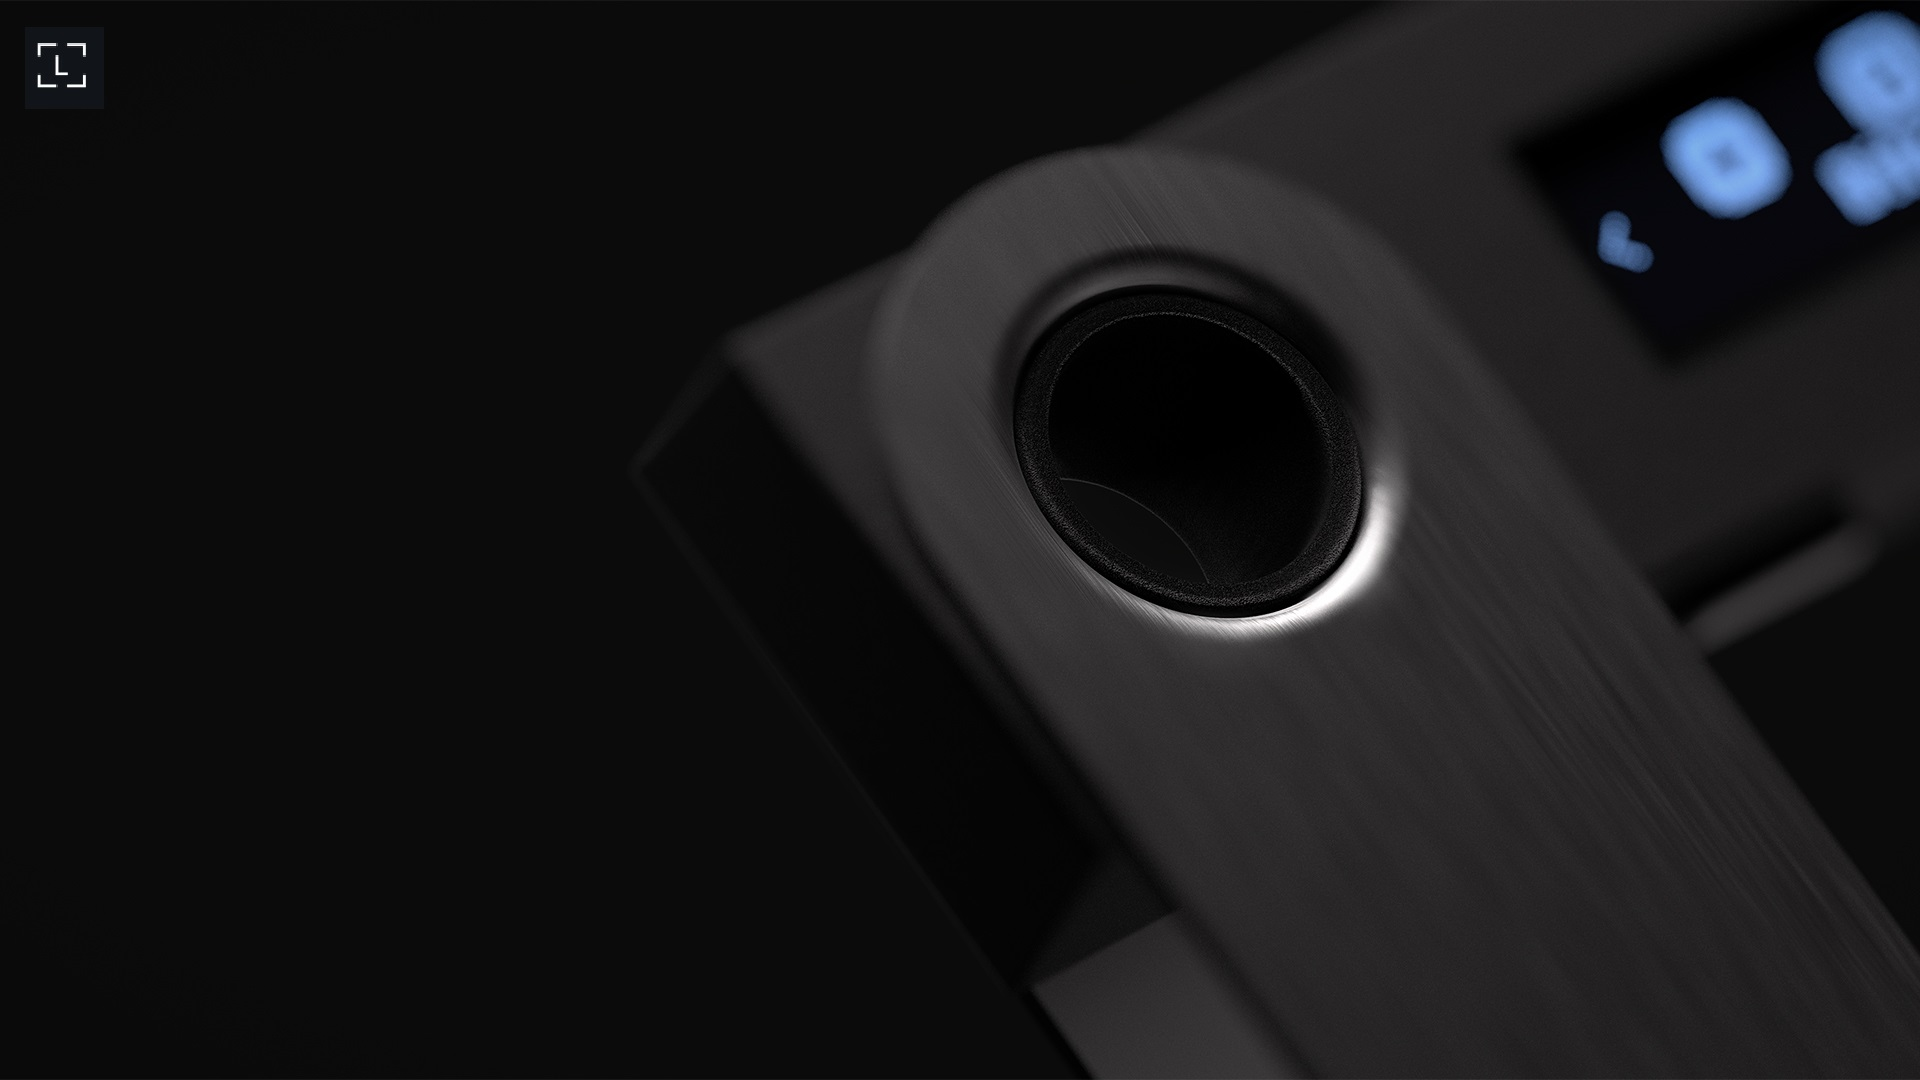
\includegraphics[width=\paperwidth,height=\paperheight]{images/fond1.jpg}
    }
\title{Multi And Threshold Signatures for Starknet} %->->->->-> Check hyperref title <-<-<-<-<-
\subtitle{(Warming up for Lisbon Hackhaton)}
\author[R. Dubois]{\textcolor{yellow}{Renaud Dubois}}
\institute[LIT]{
    \textcolor{white}{Ledger}%
    \\%
    \textcolor{white}{Innovation Team}%
} %You can change the Institution if you are from somewhere else
\date{\today}
%\logo{\includegraphics[width= 0.05\textwidth]{images/logo.png}}

\begin{document}
    
    \frame{\titlepage}
%%%%%%%%%%%%         
    \begin{frame}{Summary}
     
     \only<1>
     {
     \begin{center}
     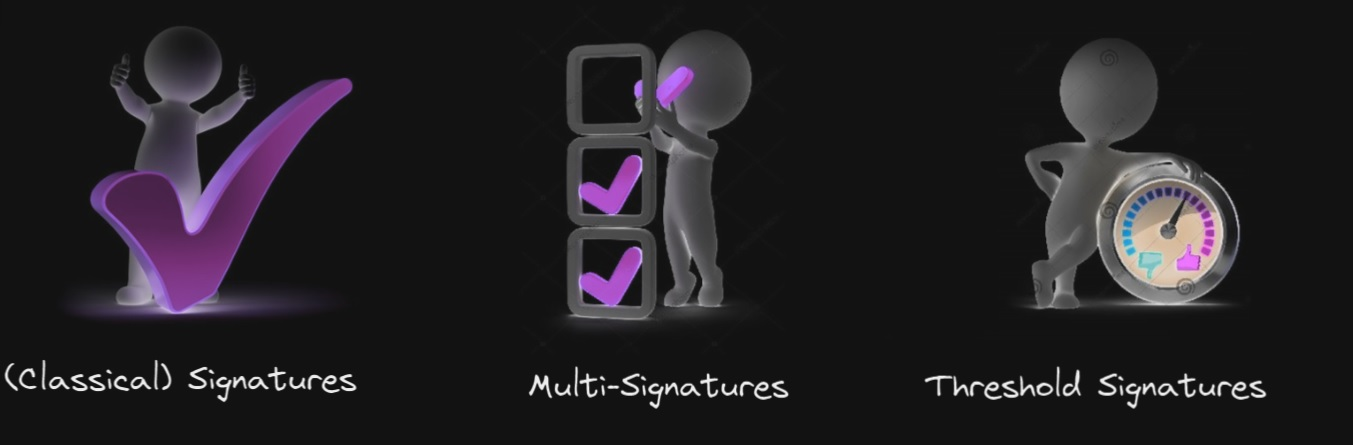
\includegraphics[width=12cm]{images/concepts.jpg}
     \end{center}
     }
     \only<2>
     {
        \tableofcontents
      }  
%         Reed-Solomon Proximity (RP) Problem: Given oracle access to a Reed-Solomon code $f:S\rightarrow\mathbb{F}$, the Reed-Solomon Proximity Problem asks that a verifier $V$ distinguishes between two cases with high probability: \begin{itemize}
%                                                                                                                                                                                                                                           \item $$f\in \textbf{RS}[\mathbb{F},S,\rho]$$
%                                                                                                                                                                                                                                           \item $f$ is $\delta$-far pairwise Hamming distance from all $$f^\prime\in\textbf{RS}[\mathbb{F},S,\rho], f\neq f^\prime$$.
%                                                                                                                                                                                                                                          \end{itemize} 
   
    \end{frame} 
%%%%%%%%%%%% 
   \section{Signatures, MultiSigs and ThresholdSigs }
    %\frame{\sectionpage}
    \subsection{Basic Concepts}
%%%%%%%%%%%%%%%%%%%%%%%%%%%%%%%%%%%%%%%%%%%%%%%%    
    \begin{frame}{Signatures}
     
%      \begin{definition}[Wikipedia]
%      Identity is the qualities, beliefs, personality traits, appearance, and/or expressions that characterize a person or group.
%      \end{definition}
     A digital signature is a mathematical scheme for verifying the authenticity of digital messages or documents.
     
     \begin{definition}[(Classical) Digital Signature]
     A signature scheme is a tuple of function:
     \begin{itemize}
     \item $Setup$: returns $E(F_p), G, H$
     \item $KeyGen(E(F_p), G, H, seed)$: returns $(pvk,pubk)=(x,Q)$
     \item $Sign(x,message)$: returns $Sig$ 
     \item $Verify(Sig,Q)$: returns {\tt true/false}
     \end{itemize}
     
     \end{definition}
     Most commonly used signature scheme is ECDSA (Bitcoin, Ethereum)
     \begin{itemize}
     \item implemented in Starknet/\href{https://github.com/starkware-libs/cairo-lang/tree/master/src/starkware/cairo/common}{\cyan{Cairo}} (P256, NTT/Stark friendly Starknet Curve)
     \item available in your favorite sdk
     \href{https://developers.ledger.com/docs/nano-app/crypto-api/ox__ec_8h/}{\cyan{Ledger}}
     
     \end{itemize} 
    
\end{frame}
%%%%%%%%%%%%%%%%%%%%%%%%%%%%%%%%%%%%%%%%%%%%%%%%
 \begin{frame}{Signatures}
 How to aggregate several authenticators into one authentication to a smart contract ?
 \begin{center}
        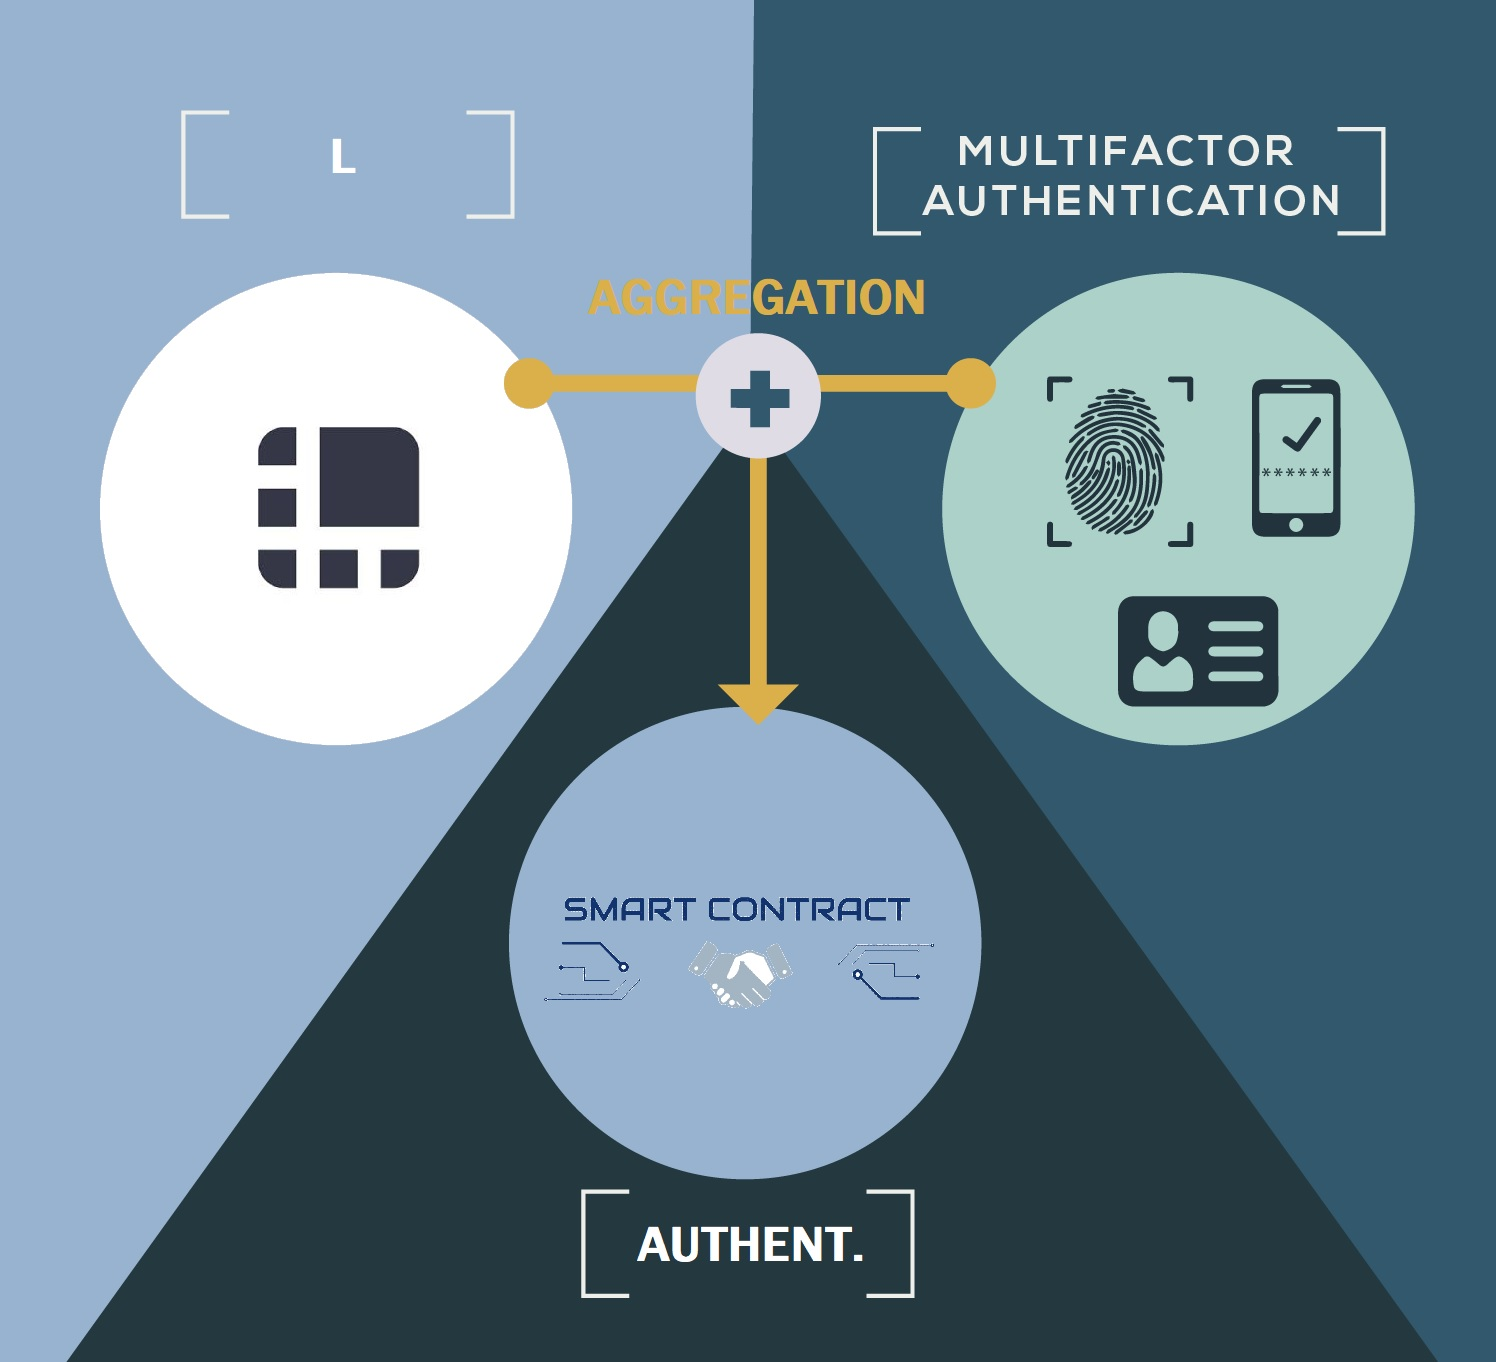
\includegraphics[width=7cm]{images/2fa.jpg}
        \end{center}
  
 \end{frame}
%%%%%%%%%%%%%%%%%%%%%%%%%%%%%%%%%%%%%%%%%%%%%%%%
  \begin{frame}{Multi-signatures}
 A multi-signature is a digital signature allowing users to {\it aggregate} their keys in an aggregated public key. The signatures are also aggregated.
  Verifier API is unchanged.
  
  
  \only<1>{
  \begin{center}
        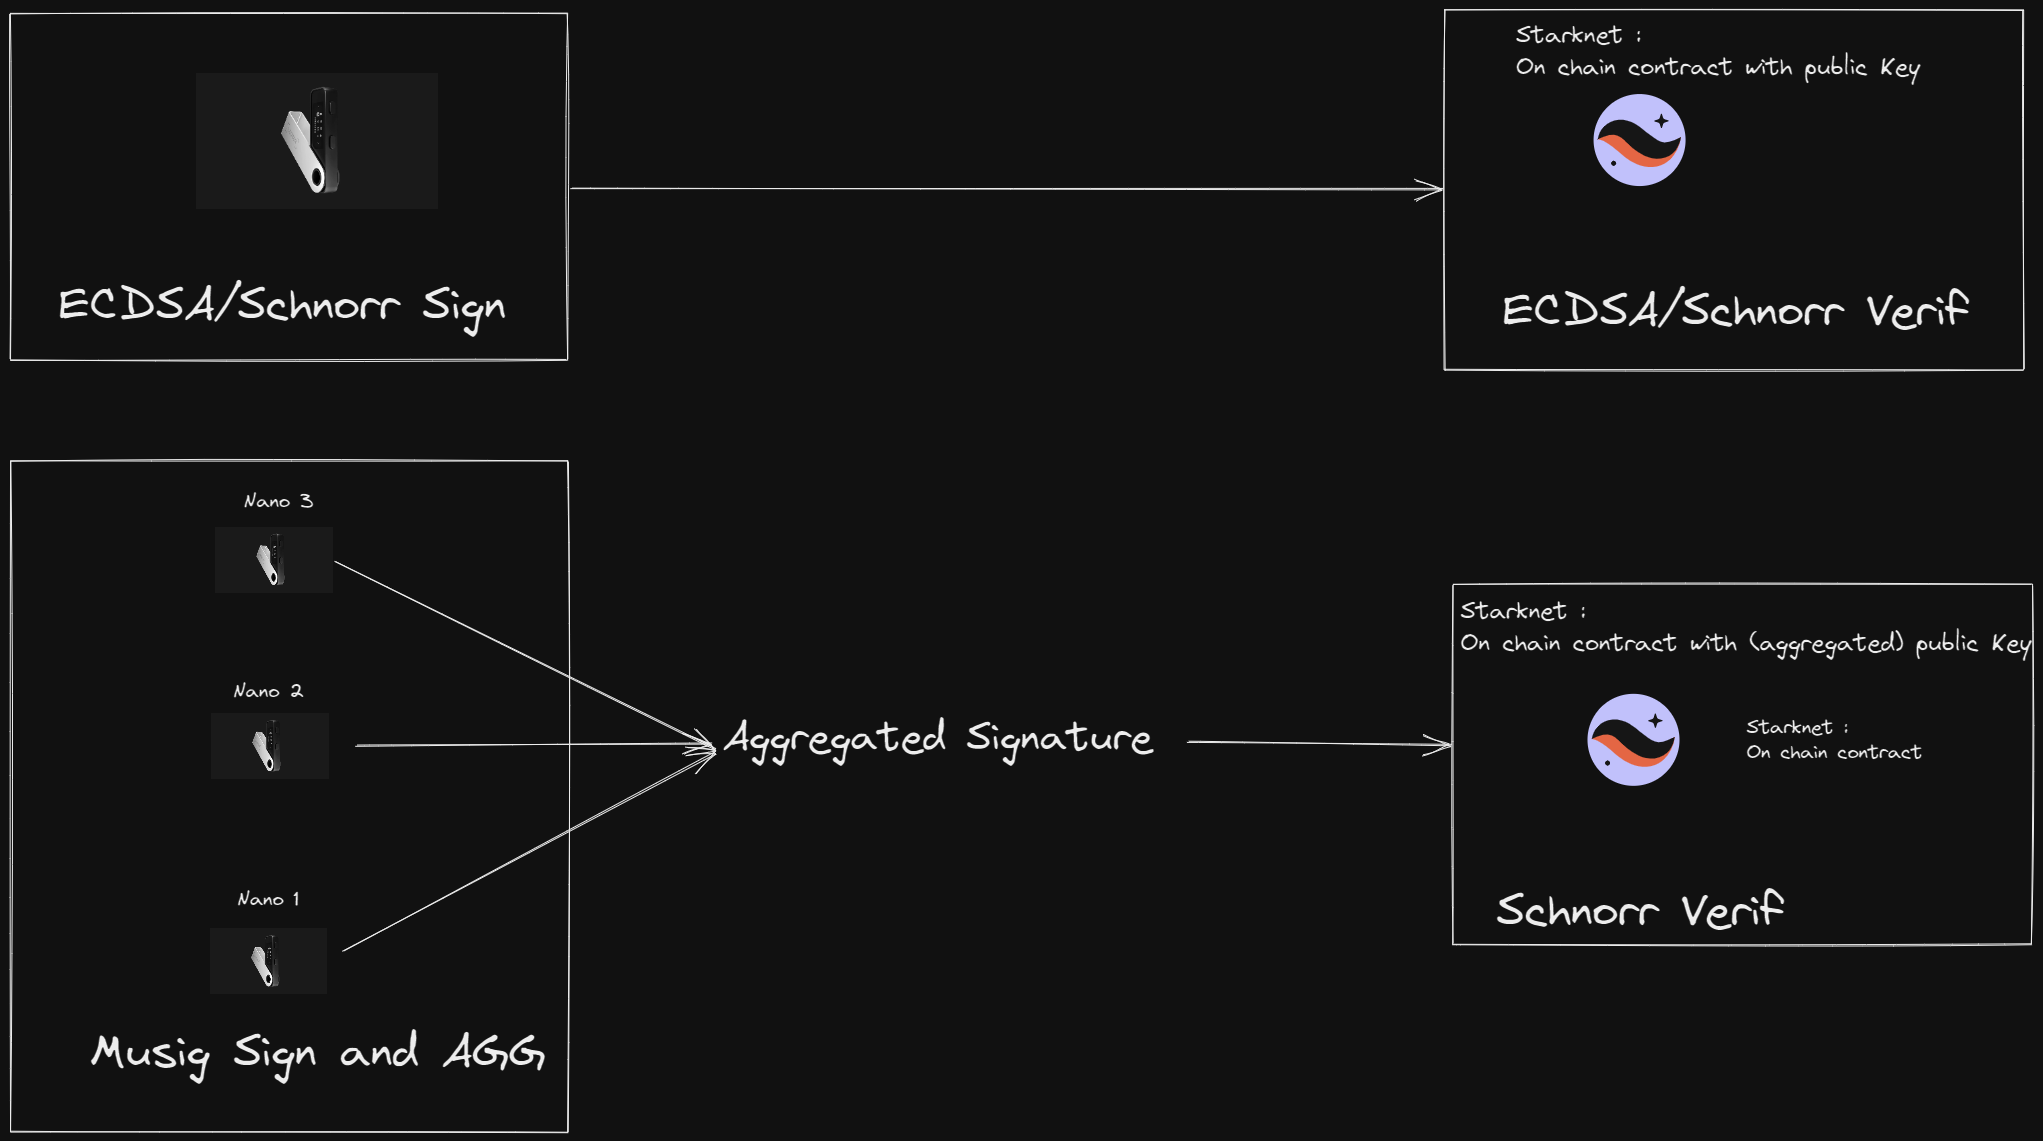
\includegraphics[width=11cm]{images/aggregate.png}
        \end{center}
  }
  \only<2>{
   \begin{definition}[(Classical) Digital Signature]
     A multisig scheme is a tuple of function:
     \begin{itemize}
     \item $(Setup, Keygen, Verify, Sign)$
     \item $KeyAgg(Q_1, \ldots Q_n)$ returns $X$
     \item $SignAgg(Sig_1, \ldots, Sig_n)$ returns $Sig$
     \end{itemize}
  \end{definition}
  }
  \only<3>
  {
  \begin{exampleblock}{Advantages (over naive concatenation/trusted aggregator)}
  \begin{itemize}
  \item only one signature over channel (bandwidth consumption)
  \item no need for a trusted aggregator (no remote private key, own your crypto !)
  \item no risk of contract failure (don't trust, no don't)
  \item verifier doesn't need to know the underlying group of users
  \end{itemize}
  \end{exampleblock}
  
  Example: Bitcoin Taproot, \href{https://en.bitcoin.it/wiki/BIP_0340}{\cyan{BIP340}}
  }
  \only<4>
  {
  \begin{alertblock}{drawback}
   \begin{itemize}
  \item requires Schorr (not in FIDO, not NIST,  
  \item increased computational complexities for signers
  \item requires (off chain) communications between signers  
  \item computation in 2 rounds (Sig1, Sig2)

\begin{center}
  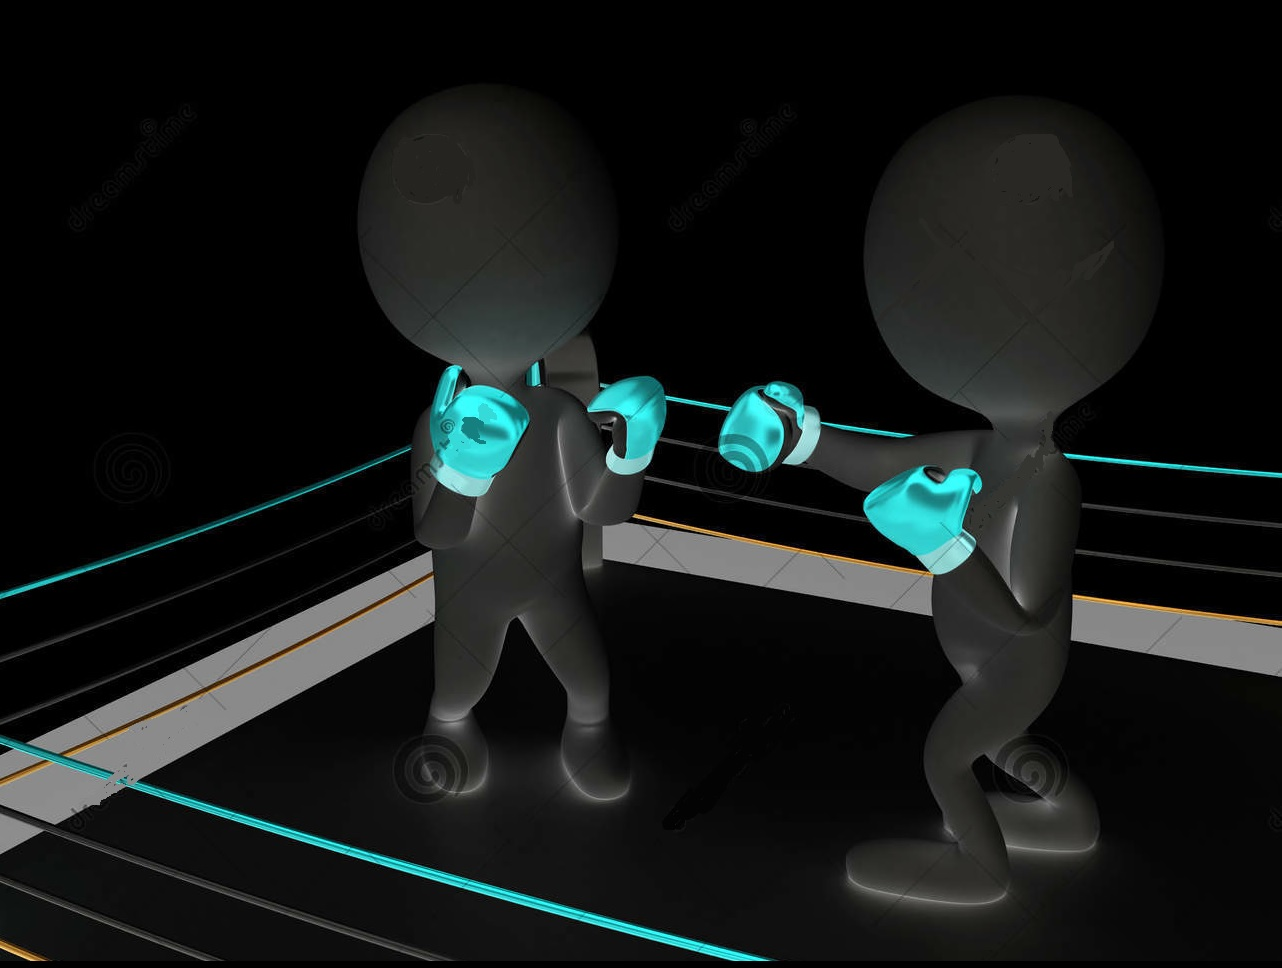
\includegraphics[width=4cm]{images/rounds.jpg}
  \end{center}
  \end{itemize}
  \end{alertblock}
  } 
 
 \end{frame}
 

%%%%%%%%%%%%%%%%%%%%%%%%%%%%%%%%%%%%%%%%%%%%%%%%
 
\begin{frame}{Threshold-signatures}


 A $(k,n)$ threshold signature (TS-Sig) is a digital signature allowing a subset (threshold) of $k$ users from $n$ to {\it aggregate} a signature . 
 
  \only<1>
  {
   \begin{center}
        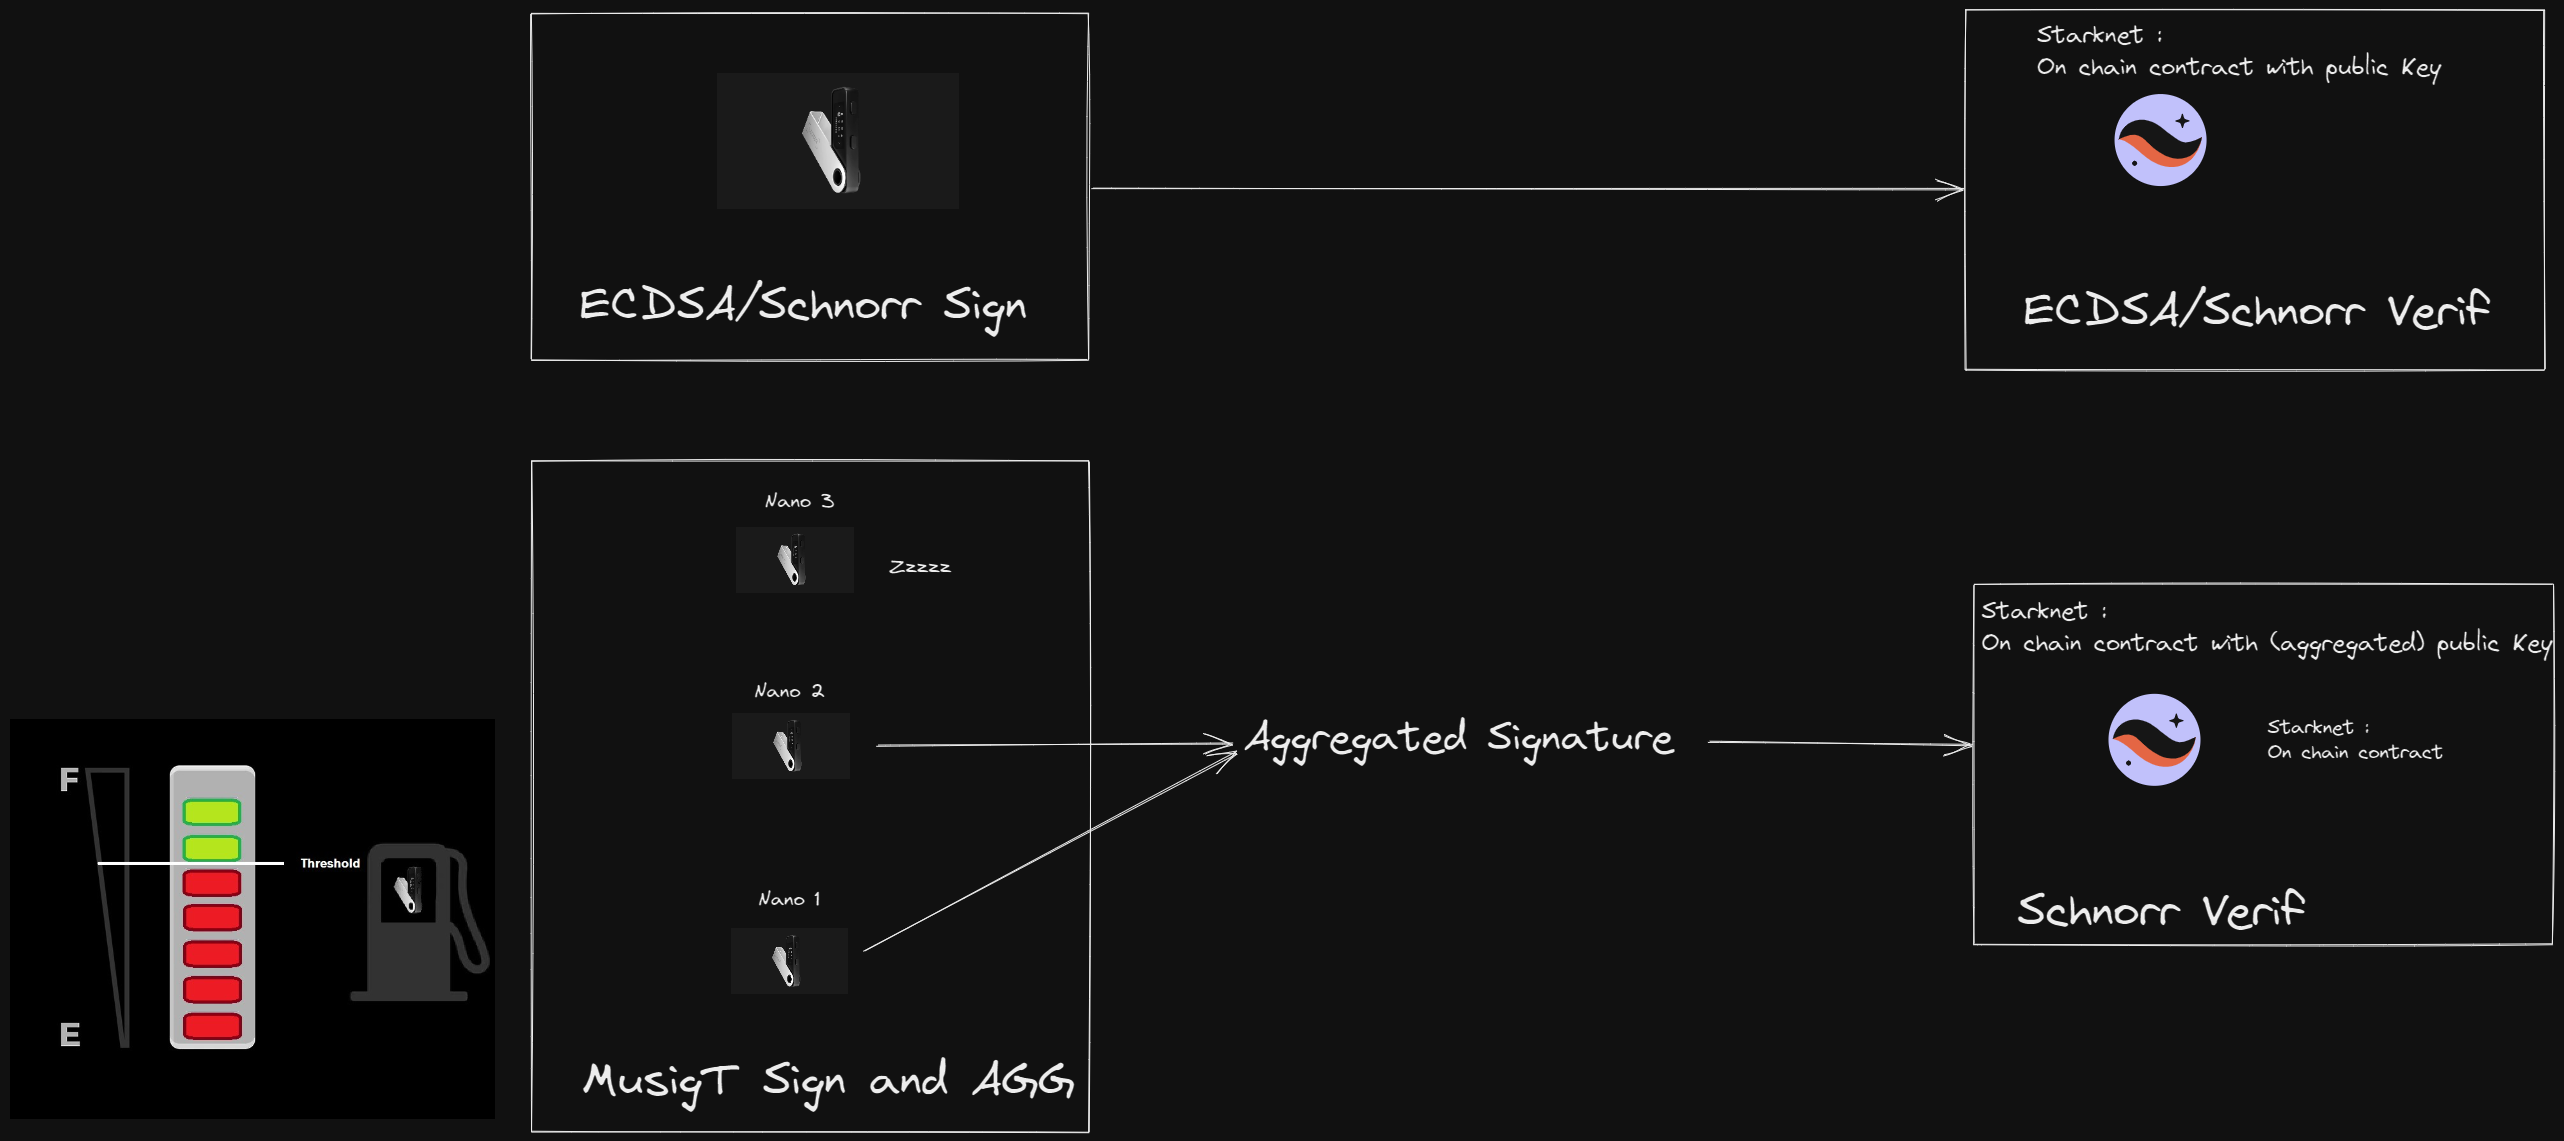
\includegraphics[width=12.2cm]{images/threshold.png}
        \end{center}
  }
  \only<2>
  {
    \begin{definition}[(Classical) Digital Signature]
     A multisig scheme is a tuple of function:
     \begin{itemize}
     \item $(Setup,  Verify, Sign)$
     \item $Distributed Keygen$,
     \item $KeyAgg(Q_1, \ldots Q_n)$ returns $X$
     \item $SignAgg(Sig_1, \ldots, Sig_n)$ returns $Sig$
     \end{itemize}
  \end{definition}
     
      {
      
  \begin{exampleblock}{Advantages (over naive concatenation/trusted aggregator)}
  \begin{itemize}
  \item All of multisig ($k=n$ is equivalent)
  \item More flexibility in access policy
  \end{itemize}
  \end{exampleblock}
 
  } 
   Example: FROST(Blockstream).
 }
\end{frame}
%%%%%%%%%%%%%%%%%%%%%%%%%%%%%%%%%%%%%%%%%%%%%%%%
 \subsection{Under the hood}

\begin{frame}{Disclaimer}

 \begin{center}
 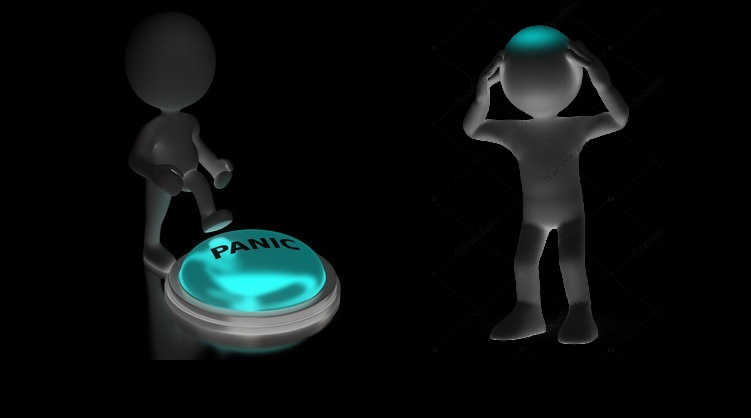
\includegraphics[width=12.2cm]{images/panic.jpg}
 \end{center}


\end{frame}
 

\begin{frame}{EC-Schnorr and ECDSA}

SetUP() : Pick a \href{https://github.com/LedgerHQ/speculos/blob/master/src/bolos/cx_ec_domain.c}{\cyan{curve}} with parameters $(p,a,b,Gx,Gy,q)$ (\href{https://hyperelliptic.org/EFD/g1p/auto-shortw.html}{\cyan{ weierstrass equations and formulaes}} ).

  \begin{center}
\begin{tabular}{|c|c |c|}
\hline
Operation&
\includegraphics[width=1cm]{images/schnorr.jpg} & ECDSA \\
\hline
KeyGen &$Q=xG$        &$Q=xG$ \\

Nonce$^*$&$k$	&  $k$ \\
Ephemeral&$R=kG$    &$R=kG$  \\
\hline

Hash &$e=H(m||R)$ & $e=H(m)$\\
\hline

Sign &$s=k-xe$    & $s=k^{-1}(e+xr)$  \\
     & $Sig=(R,s)$ & $Sig=(r,s)$ \\	
\hline
Verif &   $R'=sG+eQ$& $r'=(es^{-1}G+rs^{-1}Q)_x $ \\    
      & Accept if R'=R & Accept if r'=r \\
\hline
\end{tabular}  
 \end{center}
 
 
 \begin{center}
 \begin{small}
 {\emph{
 (* nonce generation may use \href{https://www.rfc-editor.org/rfc/rfc6979}{\cyan{RFC6979}} for misuse resistance)}}
 \end{small}
\end{center}

\end{frame} 
 

%%%%%%%%%%%%%%%%%%%%%%%%%%%%%%%%%%%%%%%%%%%%%%%%

\begin{frame}{Musig2: using Schnorr additive properties}

   
       

\only<1>
{  

Schnorr s part is linear in $(k,x)$ and {\red linerarity} is cool:
\begin{tabular}{lllr}
$s(k,x_1)+Sig(k,x_2)$&$=$& $s(k, x_1+x_2), $&$\forall  x=x_1+ x_2$\\
$s(k_1,x)+Sig(k_2,x)$&$=$& $s(k, x), $&$\forall k=k_1+ k_2$\\
\end{tabular}

(while ECDSA has degree two monomial in $(k,x)$)

 \begin{center}
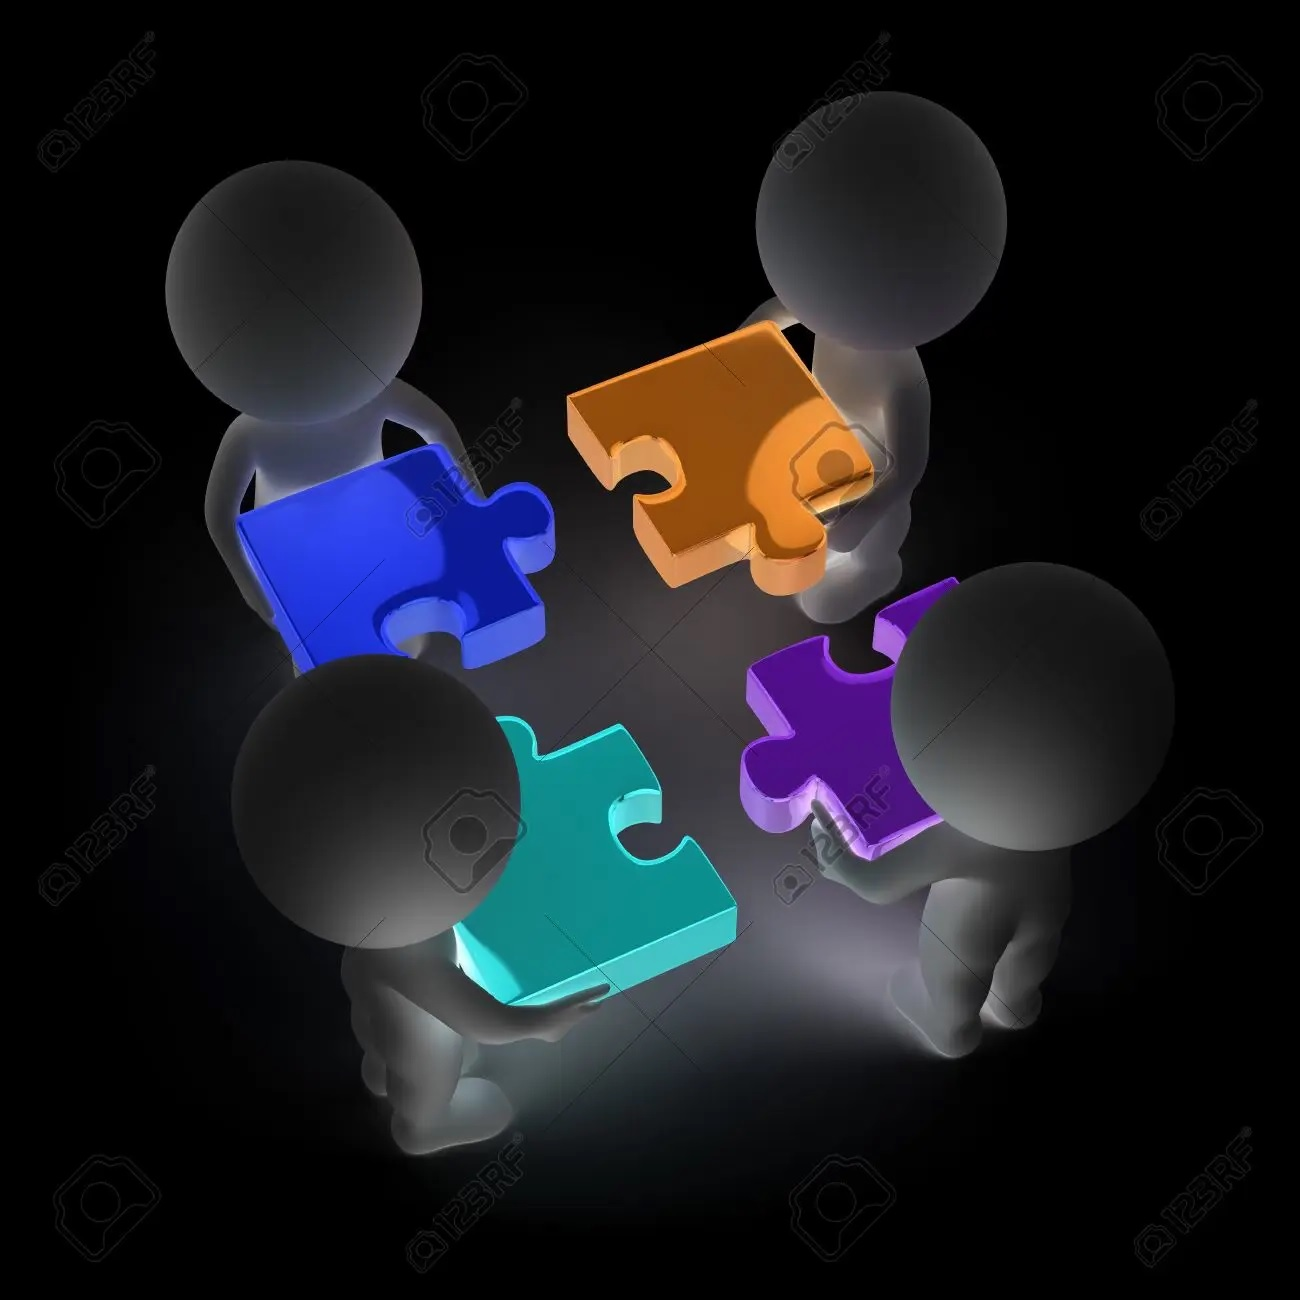
\includegraphics[width=4cm]{images/multi3d.jpg}
\end{center}
     
     
Linearity allow homomorphic additions. Idea: split X into $X=\sum a_iX_i$, k into $k=\sum k_i$.
    
}

\only<2>
{

  \begin{center}
\begin{tabular}{|c|c |c|}
\hline
Operation&Schnorr & Insec\_Musig \\
\hline
KeyGen &$X=xG$       & $X_i=x_iG$ \\
{\red KeyAgg} & - & X=$\sum_{i=0}^{n-1} a_iX_i$ \\
Nonce$^*$&$k$	&  $k_i$ \\
Ephemeral&$R=kG$   & $R_i=k_iG$ \\
{\red Aggregate R}   & -     & $R=(\sum_{i=0}^{n-1} a_i.k_i).G=k.G$\\
Hash &$e=H(m||R)$ & $e=H(m||R)$\\
Sign &$s=k-xe$    & $s_i=k_i-a_ix_ie$  \\
{\red Aggregate s} & - & $s=\sum s_i = k-xe$ \\
\hline
\end{tabular}  
 \end{center}
 
 }
 
\only<3>
{  
Musig2 uses a vectorial nonce of length $\mu$, injected in previous Insec\_Musig scheme.

  \begin{center}
\begin{tabular}{|c|c |c|}
\hline
Operation&Schnorr & Musig2 \\
\hline
KeyGen &$X=xG$       & $X_i=x_iG$ \\
{\red KeyAgg} & - & X=$\sum_{i=0}^{n-1} a_iX_i$ \\
Nonce$^*$&$k$	&  $\vec{k_i}=(k_{i1}, \ldots , k_{i\mu})$ \\
Ephemeral&$R=kG$   & $\vec{R_i}=\vec{k_i}G$ \\
Hash Nonce & - & $b=H(X||R_0 \ldots R_\mu ||m)$\\

{\red Aggregate R}   & -     & $R=\sum_{j=1}^\mu b^{j-1} (\sum_{i=0}^{n-1} a_i.k_i).G=k.G$\\
Hash &$e=H(m||R)$ & $e=H(m||R)$\\
Sign &$s=k-xe$    & $s_i=(\sum_{j=1}^\mu k_ijb^{j-1} )-a_ix_ie$  \\
{\red Aggregate s} & - & $s=\sum s_i = k-xe$ \\
\hline
\end{tabular}  
 \end{center}
  
  
}
\end{frame}
  
%%%%%%%%%%%%%%%%%%%%%%%%%%%%%%%%%%%%%%%%%%%%%%%%

\begin{frame}{Musig2: Thresholdisation Principle}

\only<1>
{
Thresholdisation use the principle of \href{https://dl.acm.org/doi/10.1145/359168.359176}{ \cyan{Shamir's secret sharing scheme }}, which is in fact a reed solomon erasure code.

Goal: Given enough shares, it is possible to reconstruct the initial value.

\begin{center}
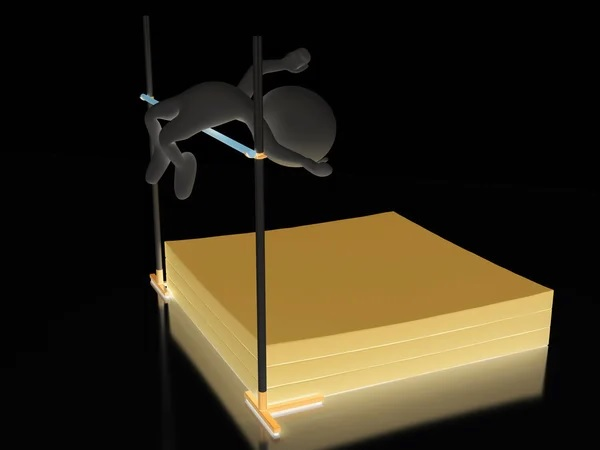
\includegraphics[width=4cm]{images/jump.jpg}
\end{center}            

}
\only<2>
{
Lagrange interpolation enables to switch from points to polynomial coefficients using the following formulaes:

\begin{center}
\begin{tabular}{cc}

\begin{minipage}{4cm}
\begin{center}
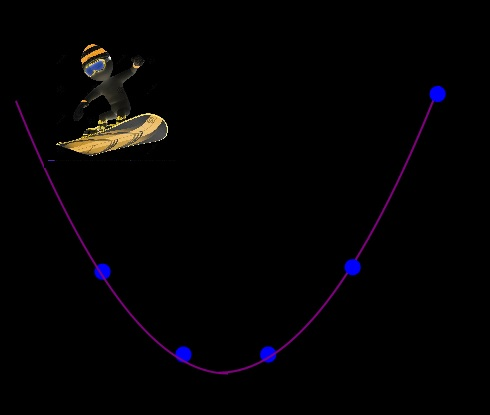
\includegraphics[width=4cm]{images/interpolation.jpg}
\end{center}            
\end{minipage}
&         
\begin{minipage}{4cm}
$$l_j(x)=\prod_{m\ne j}{x-x_m \over x_j-x_m}.$$
$$L(x)=\sum_{j=0}^k P(x_j)l_j(x).$$
\end{minipage}         
\\
\end{tabular}
\end{center}
The transformation L from $(P_0 \ldots P_k)$ to $(a_0 \ldots a_k)$ is a {\red linear} transformation in x.

\vskip+1cm
{\emph{Sidenote: This is closely related to the principle of FRI used in starks.}}

}
\only<3>
{
Key ideas:
\begin{itemize}
\item interprete aggregated secret key as a polynomial $P$ of degree $k$,
\item each share (user secret key) is a point of the polynomial,
\item blind the computation in the curve domain to perform the aggregation only handling public elements,
\item replace '$\sum_{i=0}^n$' in previous scheme by Lagrange polynomials,
\item some more steps are necessary (commitments) to avoid cheating.
\end{itemize}

Read \href{https://eprint.iacr.org/2020/852.pdf}{{\cyan FROST}} for full description.

}



\end{frame}  

%%%%%%%%%%%%%%%%%%%%%%%%%%%%%%%%%%%%%%%%%%%%%%%%


 \section{Use cases}
 
\subsection*{You survived !}
 
 
 
\begin{frame}{Use cases}


\begin{center}
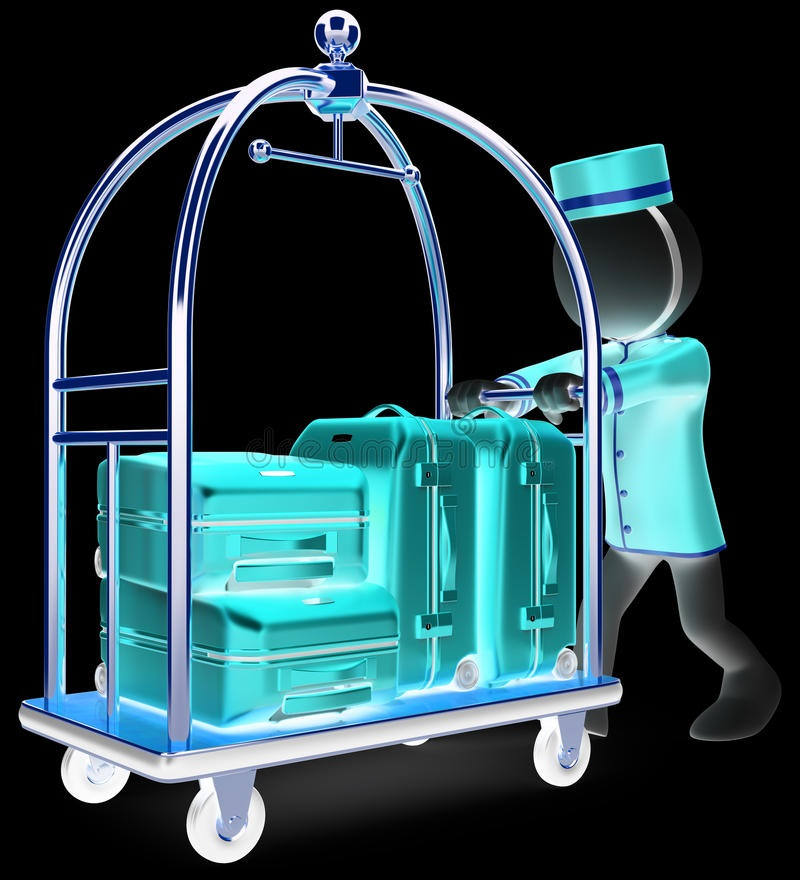
\includegraphics[width=6cm]{images/usecases.jpg}
\end{center}           

\end{frame}


\subsection{Multi factor authentication}

\begin{frame}{Multi factor authentication to Starknet Contract}
Implement enhanced policy access to assets.

\begin{center}
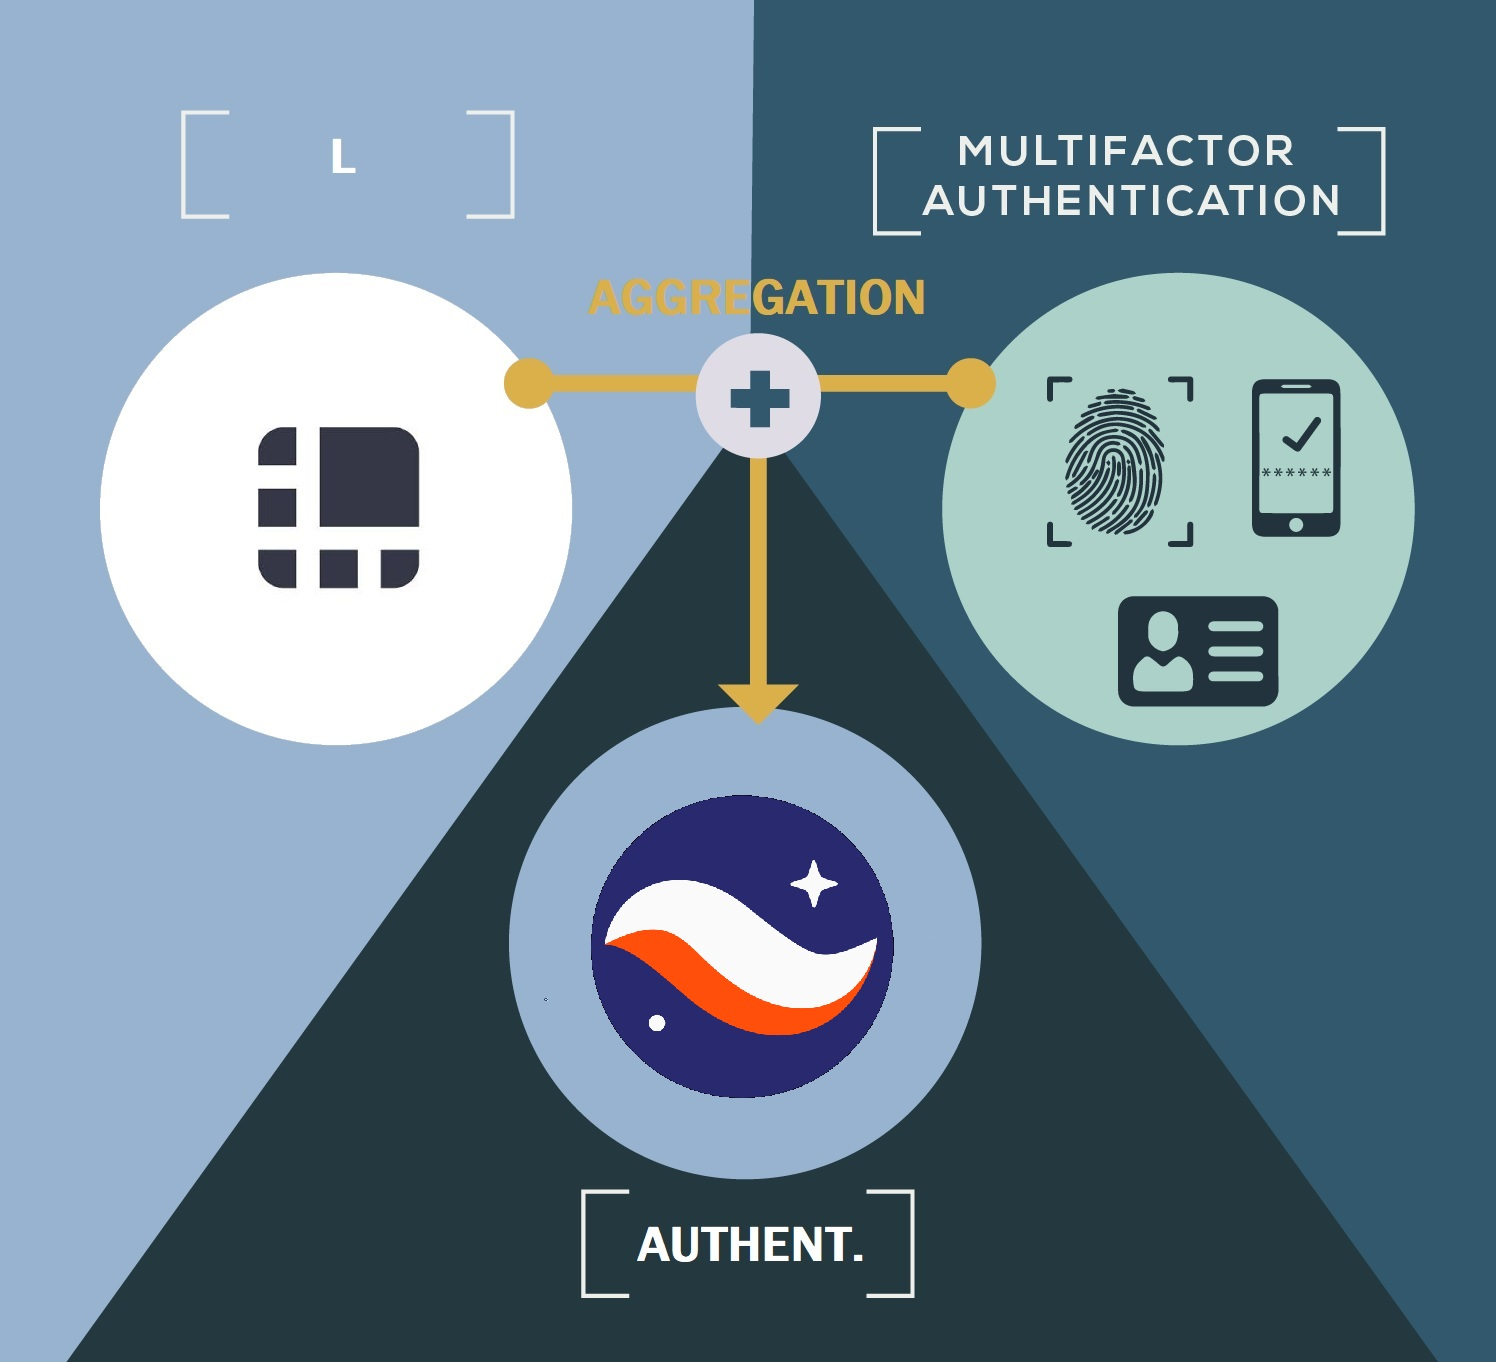
\includegraphics[width=4cm]{images/2fa2.jpg}
\end{center}

\begin{exampleblock}{Access Policy}
\begin{itemize}
\item Low amount: Host (hot wallet) only
\item High amount: Host (smartphone) + HW wallet (Nano) 
\end{itemize}
\end{exampleblock}
Use WebAuthn (FIDO) into Starknet ?

\end{frame} 

\subsection{Voting system}

%%%%%%%%%%%%%%%%%%%%%%%%%%%%%%%%%%%%%%%%%%%%%%%%
\begin{frame}{Voting system}
Reduce risk and complexity of a contract implementing a voting system.
A vote is adopted only though a valid TS-Sig.


\begin{center}
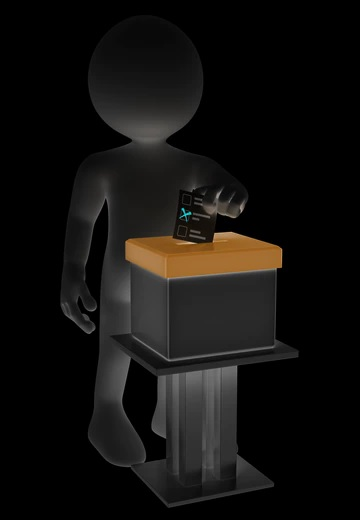
\includegraphics[width=2cm]{images/vote.jpg}
\end{center}

\begin{exampleblock}{Gnosis advanced}
\begin{itemize}
\item implement a threshold voting system, with $k={n\over 2}$
\end{itemize}
\end{exampleblock}


\end{frame} 

%%%%%%%%%%%%%%%%%%%%%%%%%%%%%%%%%%%%%%%%%%%%%%%%
\section{Ledger/Starknet Musig2, call for Lisbon}


%%%%%%%%%%%%%%%%%%%%%%%%%%%%%%%%%%%%%%%%%%%%%%%%

\begin{frame}{Ledger/Starknet Musig2}

Specificities of Musig2 Starknet (ease Prover/Verifier computations)
\begin{itemize}
\item Addition of EC-Schnorr to Cairo contracts
\item Uses Pedersen Hash as core hash function 
\item Uses Starknet curve as elliptic domain
\item Implement x-only verification
\end{itemize} 
The implementation is a generic one (takes hash and elliptic domain as SetUp parameter).
The aim is to overlap 
\begin{itemize}
\item with B340 if selecting P256k1 and SHA256 instead (TBD).
\item with \href{https://datatracker.ietf.org/doc/html/draft-irtf-cfrg-eddsa-05}{{\cyan RFC Eddsa}} if selecting Ed25519.        
\end{itemize}

     
\end{frame}

%%%%%%%%%%%%%%%%%%%%%%%%%%%%%%%%%%%%%%%%%%%%%%%% 
\begin{frame}{Ledger/Starknet Musig2}

\only<1>
{
\begin{exampleblock}
{Current state}
\begin{itemize}
\item Schnorr verification available in Cairo, 
\item High-level simulation in Sagemath of full protocol (Sign/Verify for a pool of users) 
\item Musig2 implementation on top of a virtualization layer (only integrating bolos for now) 
\item currently working on thresholdization
\end{itemize} 
\end{exampleblock}
}
\only<2>
{

\begin{alertblock}
{Next steps}
\begin{itemize}
\item Thresholdisation,
\item Compatibility with Edd25519 (FIDO compliance) 
\begin{center}
 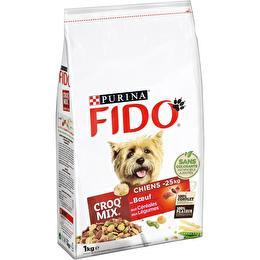
\includegraphics[width=2cm]{images/fido.jpg}
 \end{center}
\end{itemize}

\end{alertblock}
}

     
            \begin{tabular}{ccc}
           \href{https://github.com/rdubois-crypto/CYLIB-Speculos}{\cyan{C Library (Nano Signer)}} &~~~~~~~~~~~~~~~ &   \href{https://github.com/rdubois-crypto/MyCairoPlayground}{\cyan{Cairo Code (Contract Verifier)}}\\
            
           
\includegraphics[width=2cm]{images/musig2_qr.jpg} & ~~~~~~~~~~~~~~~&
\includegraphics[width=2.1cm]{images/cairomusig2_qr.jpg}
            \\
           \end{tabular}     		
\end{frame} 

%%%%%%%%%%%%%%%%%%%%%%%%%%%%%%%%%%%%%%%%%%%%%%%%

\begin{frame}{Starknet Hackhaton}

\begin{center}
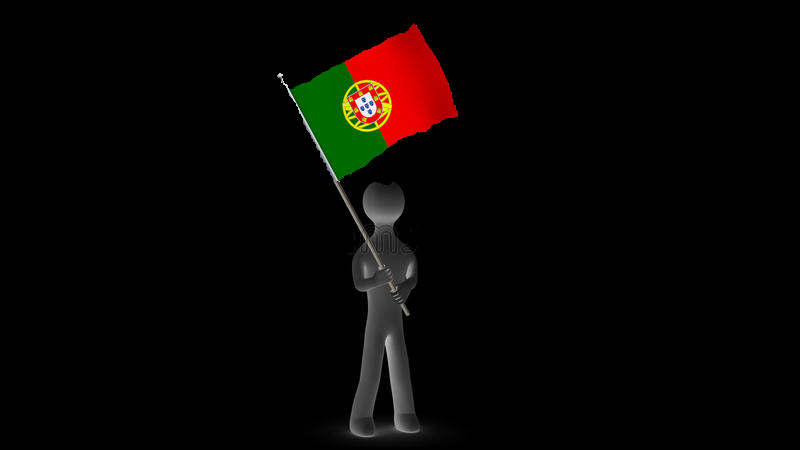
\includegraphics[width=6cm]{images/lisbon.png}
\end{center}

Join the team for:
\begin{itemize}
\item Front end integration (wallet, current development over Argent) over verifier (Cairo) or signer (C)
\item Integration of a different accelerator/library in the virtualization layer (C)
\item Contribute to the threshold version (Sagemath/C)
\end{itemize} 

\end{frame} 
%%%%%%%%%%%%%%%%%%%%%%%%%%%%%%%%%%%%%%%%%%%%%%%%
    \section{}
    \begin{frame}{}
        \centering
            {\Huge\bfseries
        \textcolor{yellow}{Questions ?}}
        
            
\includegraphics[width=8cm]{images/questions.jpg}
            
           \begin{tabular}{ccc}
           \href{https://github.com/rdubois-crypto/CYLIB-Speculos}{\cyan{C Library}} & ~~~~~~~~~~~~~~~~~~\href{https://github.com/rdubois-crypto/MyCairoPlayground/tree/main/slides}{\cyan{Slides }} ~~~~~~~~~~~~~~~~~~&   \href{https://github.com/rdubois-crypto/MyCairoPlayground}{\cyan{Cairo\&Sage }}\\
            
           
\includegraphics[width=2cm]{images/musig2_qr.jpg} & 
\includegraphics[width=2.1cm]{images/qrslides.jpg} &
\includegraphics[width=2.1cm]{images/cairomusig2_qr.jpg}
            \\
           \end{tabular}     		
    \end{frame}
\end{document}

  
% https://en.wikipedia.org/wiki/Privacy
% [CL16]: Concepts Around Privacy-Preserving Attribute-Based CredentialsJan Camenisch  https://hal.archives-ouvertes.fr/hal-01276046/document
